\subsection{Balance Scale}

\subsubsection{Backpropagation padrão}

O backpropagation padrão foi executado para a base de dados Balance Scale com os seguintes parâmetros:

\begin{itemize}
	\item \texttt{size}: 5
	\item \texttt{learnFuncParams}: 0.1
	\item \texttt{maxit}: 50
\end{itemize}

A confusion matrix de uma execução é apresentada na Figura \ref{figura-confusion-matrix-balance-scale-backpropagation-padrao}.

\begin{figure}[h!]
  \centering
  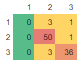
\includegraphics[width=0.3\linewidth]{figs/confusion-matrix-balance-scale-backpropagation-padrao.png}
  \caption{Confusion Matrix - Balance Scale - Backpropagation padrão}
  \label{figura-confusion-matrix-balance-scale-backpropagation-padrao}
\end{figure}

Os resultados para as 10 execuções do backpropagation padrão com as taxas de acertividade são apresentados na Tabela \ref{tabela-resultado-balance-scale-backpropagation-padrao}. A média de acertividade foi de $0.8713$, com desvio padrão de $0.0267$.

\begin{table}[h!]
\centering
\caption{Resultados - Balance Scale - Backpropagation padrão}
\label{tabela-resultado-balance-scale-backpropagation-padrao}
\begin{tabular}{ll}
\toprule
                       & \textbf{Acertividade}       \\ \midrule
Execução 1             & 0.8617          \\
Execução 2             & 0.8617          \\
Execução 3             & 0.8511          \\
Execução 4             & 0.9255           \\
Execução 5             & 0.8723          \\
Execução 6             & 0.8298           \\
Execução 7             & 0.8723           \\
Execução 8             & 0.9043          \\
Execução 9             & 0.8617           \\
Execução 10            & 0.8723           \\ \bottomrule
\textbf{Média}         & \textbf{0.8670} \\
\textbf{Desvio Padrão} & \textbf{0.0267}
\end{tabular}
\end{table}

%O erro iterativo é apresentado na Figura \ref{figura-erro-iterativo-balance-scale-backpropagation-padrao}.
%
%\begin{figure}
%  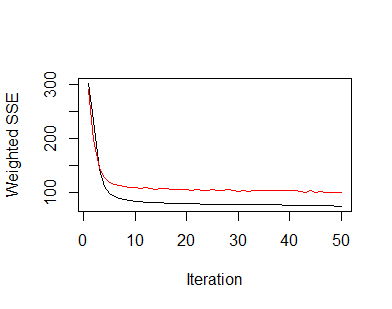
\includegraphics[width=\linewidth]{figs/erro-iterativo-balance-scale-backpropagation-padrao.png}
%  \caption{Erro iterativo - Balance Scale - Backpropagation Padrão}
%  \label{figura-erro-iterativo-balance-scale-backpropagation-padrao}
%\end{figure}

\subsubsection{SCG}

O backpropagation com função de aprendizado SCG foi executado para a base de dados Balance Scale com os seguintes parâmetros:

\begin{itemize}
	\item \texttt{size}: 5
	\item \texttt{learnFuncParams}: (0, 0, 0, 0)
	\item \texttt{maxit}: 50
\end{itemize}

A confusion matrix de uma execução é apresentada na Figura \ref{figura-confusion-matrix-balance-scale-backpropagation-scg}.

\begin{figure}[h!]
  \centering
  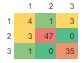
\includegraphics[width=0.3\linewidth]{figs/confusion-matrix-balance-scale-backpropagation-scg.png}
  \caption{Confusion Matrix - Balance Scale - Backpropagation SCG}
  \label{figura-confusion-matrix-balance-scale-backpropagation-scg}
\end{figure}

Os resultados para as 10 execuções do backpropagation SCG com as taxas de acertividade são apresentados na Tabela \ref{tabela-resultado-balance-scale-scg}. A média de acertividade foi de $0.9234$, com desvio padrão de $0.0425$.

\begin{table}[h!]
\centering
\caption{Resultados - Wine - Backpropagation SCG}
\label{tabela-resultado-balance-scale-scg}
\begin{tabular}{ll}
\toprule
                       & \textbf{Acertividade}       \\ \midrule
Execução 1             & 0.9149          \\
Execução 2             & 0.9043          \\
Execução 3             & 0.9574           \\
Execução 4             & 0.9255          \\
Execução 5             & 0.9574           \\
Execução 6             & 0.8191          \\
Execução 7             & 0.9574           \\
Execução 8             & 0.9468           \\
Execução 9             & 0.9468          \\
Execução 10            & 0.9043          \\ \bottomrule
\textbf{Média}         & \textbf{0.9234} \\
\textbf{Desvio Padrão} & \textbf{0.0425}
\end{tabular}
\end{table}

%O erro iterativo é apresentado na Figura \ref{figura-erro-iterativo-balance-scale-backpropagation-scg}.
%
%\begin{figure}
%  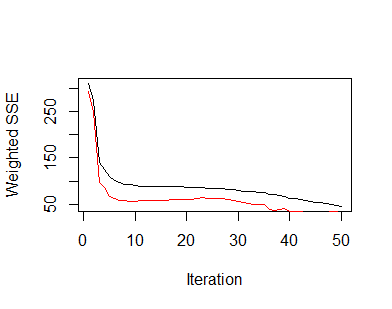
\includegraphics[width=\linewidth]{figs/erro-iterativo-balance-scale-backpropagation-scg.png}
%  \caption{Erro iterativo - Balance Scale - Backpropagation SCG}
%  \label{figura-erro-iterativo-balance-scale-backpropagation-scg}
%\end{figure}